
\section{Summary}
In this chapter, I would like to summarize the findings established at each of the chapters to summarize the entire thesis.
\\
\\
Along with CMOS scaling, wireless/wireline communication performances have greatly advanced and continues to evolve.
To realize a system on chip (SoC) for such products, high-performance ADCs are required.  
However, such SoCs utilize scaled CMOS technologies to cut down the costs of the digital circuits, but analog circuit's performance severely degrades when implemented on such processes. 
Thus, the design of ADCs in scaled CMOS process environments becomes one of the most challenging and critical fields of circuit design.

Throughout the thesis, to realize CMOS process scalable ADCs, we explored Hybrid ADCs and novel design techniques that heavily utilize successive-approximation (SA) circuitry. Our key idea was that since the SA circuitry enjoys benefits of process scaling, the ADCs which integrate SA will also become process scalable as well.
\\
\\
In chapter 2, we introduced the concept and implementation of the digital amplifier (DA) to realize a CMOS process scalable switched capacitor amplifier.
Conventionally, the amplifier (or the Opamp) gain performance greatly degraded with scaling with worsened transistor gain and lowered supply voltages and has been the greatest challenge upon scaling the Pipelined-ADCs.

We presented the DA's all error canceling feature, where the gain error, non-linearity, incomplete settling, power supply noise and thermal noise of the low-gain amplifier can be canceled out by feedback based on successive approximation. Unlike conventional amplifiers, the DA accuracy can be arbitrarily set by configuring the number of bits in the DA C-DAC; the amplifier gain is decoupled from the transistor intrinsic gain, which is suitable for scaled CMOS integration.

We also reported the measurement results of the calibration-free 0.7V 12bit 160MS/s pipelined-SAR ADC. Without any calibration, the ADC achieved SNDR of 61.1dB and FoM of 12.8fJ/conv., which achieved 3$\times$ higher power efficiency than conventional calibration-free ADCs. Also, an inter-process performance comparison was performed, where we fabricated 28nm and 65nm CMOS versions of the DA (and the Pipelined ADC) to confirm the process scalability of the DA.
Interestingly, we observed 3$\times$ improvement in the area, power, and 2$\times$ improvement in amplification speed, due to the process scalability of successive approximation circuits.
\\
\\
In chapter 3, we introduced the ADC with dynamic architecture and frequency scaling (DAFS).
An aggressive frequency power scaling high-speed ADCs are required for ultra-wideband communication systems, but simply configuring the ADC supply voltages are not feasible.
To accomplish superlinear power scaling in high-speed ADCs, we proposed a dynamic architecture and frequency scaling (DAFS): the ADC architecture was to be dynamically configured by adaptively between binary search and flash, reflecting the ADC clock-rate. The architecture configuration is triggered by monitoring the excess-delay of the conversion, and flash operation are used to cancel the excess-delay. DAFS not only improves the power scaling significantly but compensates for the transistor speed shift due to PVT variation which can be used to relax the design margin in high-speed ADCs.

We designed a 7-bit subranging ADC in 65nm CMOS, where the DAFS was applied to the sub-ADC. The DAFS operation was confirmed in the range of 820-1220MS/s. Our ADC was the first to achieve superlinear power scaling with 1GS/s high-speed operation. Compared to the ADC performance when DAFS was disabled, a maximum of 30\% power reduction was achieved. The ADC achieved peak FoM of 85fJ/conv. at 820MS/s, which is nearly a twofold improvement over the conventional subranging ADCs.
\\
\\
In chapter 4, we introduced wide-range threshold configuring comparators (TCCs), aiming to enhance the successive approximation (SA) circuitry of the ADCs presented in chapters 2 and 3, respectively.
For example, by utilizing 2-bit/step searches within the Digital Amplifier (DA) in chapter 2, the amplification speed can be significantly improved. 
While such TCCs will be useful and enhance the performance of ADCs based on successive approximation, it had a number of design issues: 1) it is difficult to implement large threshold configuring ranges. 2) TCCs typically have low power-supply-noise-rejection (PSNR), so the threshold was easily drifted with even small supply fluctuations.

We proposed a current source based TCC design which enables both wide-range threshold configurability and power supply variation resistance. 
The key technology relies on the proposed simple $V_{cm}$ biased current sources, which maintains sufficient comparator PSNR and keeps the ADC free from power supply variations over 10\%. 
To prove the effectiveness of the TCC, we implemented a 2-bit/step SAR ADC where the 2-bit/step comparison was carried out by TCCs instead of area and power-consuming C-DACs.
The prototype ADC fabricated in a 40nm CMOS achieved a 44.3dB SNDR with 6.14MS/s at a single supply voltage of 0.5V, and achieved a peak FoM of 4.8fJ/conv-step.


\section{Future research directions}
Last but not least, we would like to conclude our thesis by raising a few future research directions.
\\
\\
% 2-bit/step + デジタルアンプなどでさらなる高速化を狙う。
\begin{figure}
\centering
  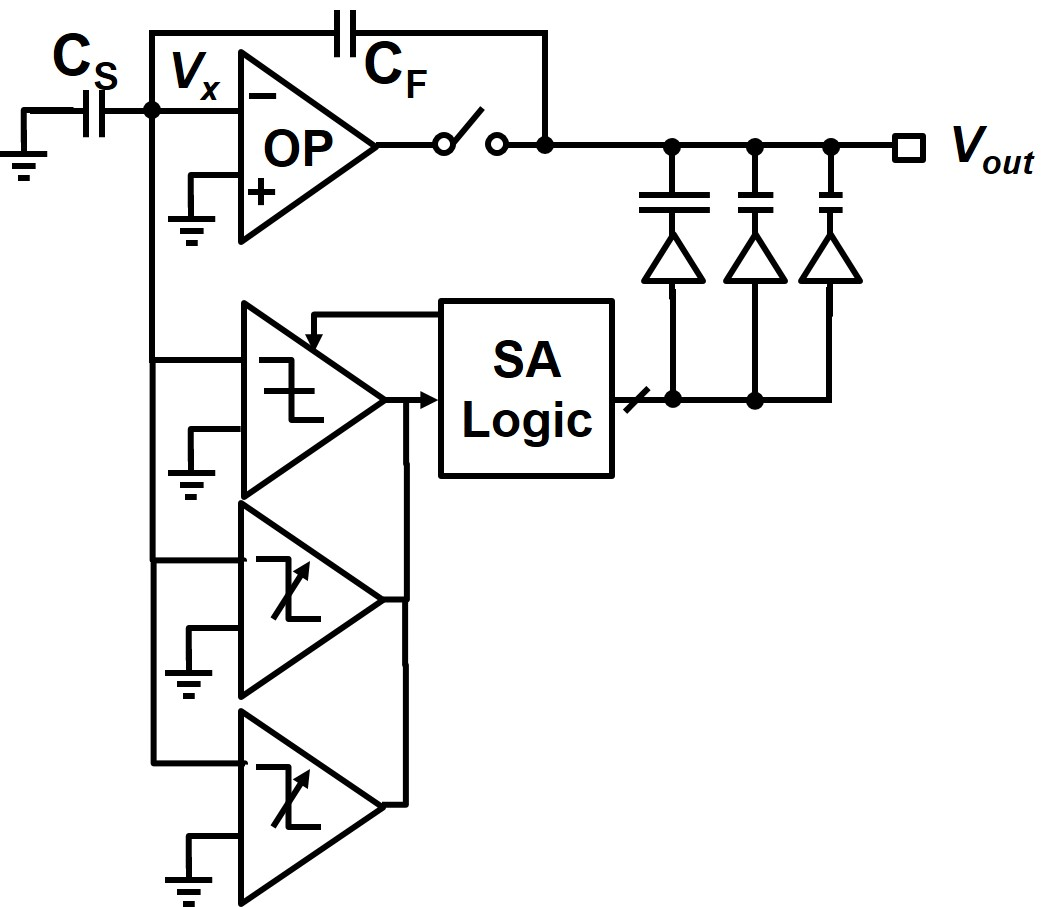
\includegraphics[width=0.7\textwidth]{figure/chap5/2bitstep.jpg}
  \caption{DA with 2-bit/step.}
  \label{fig-2bitste}
\end{figure}
The first research direction is utilizing the threshold configuring comparators (TCCs), proposed in chapter 4, to the digital amplifier.
By TCCs, we can achieve 2-bit/step SA operations to speed up the DA amplification.
Now, the total amplification time is 8ns where 2ns is allocated to the Opamp amplification and the rest 6ns is allocated to the DA.
Since 8-bit SA operation is much slower than the Opamp, 75\% of the total amplification is consumed in the DA.
By applying 2-bit/step operations as in Fig. \ref{fig-2bitste}, the SA cycle will be cut down to half: the amplification will complete within 5ns and achieve 40\% speedups.
However, by 2-bit/step the comparator count will increase three folds and calibration to set the comparator thresholds must be added, which is a non-negligible overhead. Additional techniques to null these overheads should be additionally proposed to compete for the total cost of the ADC.
\\
\\
While the above proposal was to improve the DA speeds, what can we do to further improve the DA power efficiency?
Remember that 30\% of the ADC power is still burned in the Opamp (Fig.\ref{fig-power-breakdown}).
An interesting direction will be to replace the Opamp with more efficient amplifiers (e.g. ring amplifier), the power efficiency can further be improved.
Such a fusion between ring amplifiers and digital amplifiers will be a very interesting research direction.
\\
\\
In the current digital amplifier design, the digital conversion results retrieved from the SA cycles are thrown away. Can we make good use of the conversion results the DA itself produces?
For example, if we fuse the ADC output and the DA output, we can obtain the error the Opamp generates with certain input.
Using such information, one may give feedback and calibrate the Opamp or Ringamp performance to further reduce the amplification error, similar to background calibrations.

\subsection{Further scaling the DA amplifier (down to 16nm, 7nm and beyond)}
\begin{figure}
\centering
  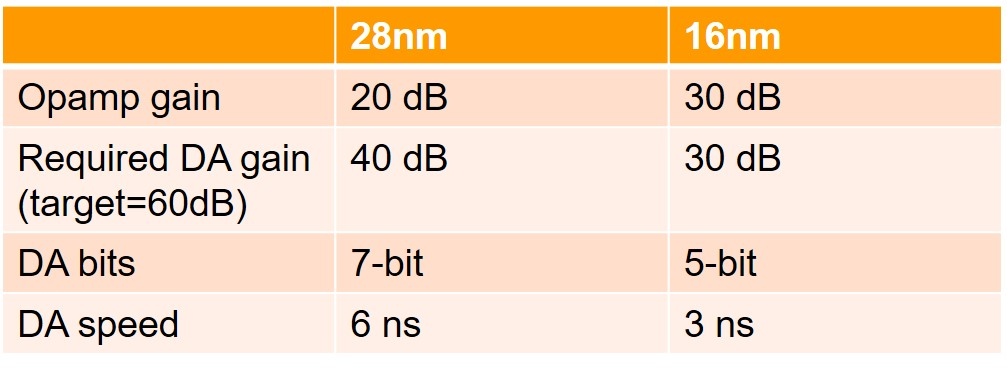
\includegraphics[width=1\textwidth]{figure/chap5/da-perf.jpg}
  \caption{DA estimated performance with 16nm and 28nm CMOS.}
  \label{fig-16nm}
\end{figure}

Does digital amplifier scale performance with even further scaled CMOS processes? And what will the DA performance look like in 16nm CMOS? 
Answering such questions will be an interesting research direction, since our thesis was to establish process scalable ADC design techniques, it will be useful to see if the proposed techniques are effective in further scaled CMOS as well.

Here, in Fig. \ref{fig-16nm}, we estimate that compared to 28nm CMOS, the 16nm CMOS with FinFETs will have 30\% fewer gate delays and also 2$\times$ higher transistor output resistances.
Interestingly, it is known by moving from planer CMOS to FinFETs, the output resistance of transistors improves since fin structures have longer effective channels.
Therefore, we estimate that the DC gains of the two-staged opamp will improve 10dB (note that we do not have access to 16nm CMOS process information and these values are only an estimate from private communication).
Thus, we can design the DA with less number of bits (e.g. 5bits), which will benefit conversion speed and power efficiency. 
Since the SA cycle speed will improve with scaling as well, we expect that the DA amplification speed will improve 2$\times$ as a whole; even designing a 320MS/s Pipelined-SAR ADC will be possible with 16nm CMOS!

While scaling down to 7nm CMOS will not improve the Opamp performance (or likely to degrade), the SA cycle speed will continue to scale and we expect higher performance in the 7nm node as well.
Since the DA will compensate for the amplifier accuracy, we estimate that one can achieve high-accuracy amplifiers even in 7nm CMOS without any gain calibration techniques. We expect a similar trend in the 5nm CMOS node as well, which is under rapid development.
